\section{Durchführung}
\label{sec:Durchführung}

\subsection{Einseitige Einspannung}

Zur Bestimmung des Elastizitätsmoduls wird eine Apparatur wie in \autoref{Abb:aufbau} verwendet. Es wird nacheinander ein Stab mit runder und quadratischer Grundfläche
wie in der Abbildung gezeigt am Punkt A eingespannt. Ein Gewicht kann nun am losen Ende des Stabes befestigt werden, wobei dieses so zu wählen ist, dass die maximale Biegung des Stabes zwischen 
3 und $\SI{7}{\milli\meter}$ liegt. Diese Biegung kann dann mit Hilfe der Messuhren und der Längenskala an jedem Punkt in Form des vertikalen Abstandes zum Auflagepunkt gemessen werden. Die Messungen
werden in einem Intervall von jeweils $\SI{3}{\centi\meter}$ mit einem Gewicht von $\SI{750}{\gram}$ durgeführt. Die verwendeten Stäbe haben dabei eine Länge von $\SI{59,3}{\centi\meter}$
(rund) und $\SI{60,2}{\centi\meter}$ (quadratisch).
Da nicht davon auszugehen ist, dass die Stäbe vor Versuchsbeginn perfekt gerade sind, werden zunächst Messungen ohne Gewicht vorgenommen.
\begin{figure}
    \centering
    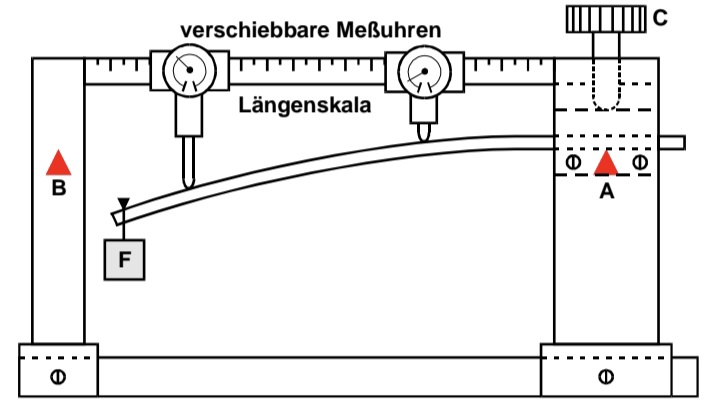
\includegraphics[width=5.5cm]{Dateien/v103Abbildung.jpg}
    \caption{Aufbau der verwendeten Messapparatur \cite{v103}.}
    \label{Abb:aufbau}
\end{figure}


\subsection{Beidseitige Auflage}
Im zweiten Teil der Messung werden die selben Stäbe nacheinander sowohl am Punkt A, als auch am Punkt B aufgelegt, jedoch ohne dabei eingespannt zu werden. Das Gewicht wird bei
diesem Aufbau in der Mitte des Stabes platziert, wobei auch hier zuvor eine Nullmessung ohne Gewicht vorgenommen wird. Die Messung der Biegung findet hierbei mit zwei verschiedenen Messuhren
statt, da durch das Gewicht in der Mitte eine durchgängige Messung mit einer Uhr nicht möglich ist.